\def\hfu{mW~m\ensuremath{^{-2}}}
\def\hgu{\ensuremath{\mu}W~m\ensuremath{^{-3}}}
\def\tcu{W~m\ensuremath{^{-1}}K\ensuremath{^{-1}}}

\chapter[Geothermics: Thermal Structure of the Earth]{Geothermics\\ {\LARGE Thermal Structure of the Earth}}\label{ch:geothermics1}
\epigraph{ ``La chaleur p{\'e}n{\`e}tre, comme la gravit{\'e}, toutes les substances de l'univers, ses rayons occupent toutes les parties de l'espace. Le but de notre ouvrage est d'exposer les lois math{\'e}matiques que suit cet {\'e}l{\'e}ment. Cette th{\'e}orie formera d{\'e}sormais une des branches les plus importantes de la physique g{\'e}n{\'e}rale.
Heat, like gravity, penetrates every substance of the universe, its rays occupy all parts of space. The object of our work is to set forth the mathematical laws which this element obeys. The theory of heat will hereafter form one of the most important branches of general physics.''}
{{\normalfont ---\ Jean-Baptiste Joseph Fourier}}

\section{Introduction}
Geothermics is the study of the distribution and transport of heat within the Earth, and occupies a distinct position among geophysical methods. Unlike gravity, magnetics, electromagnetics, and seismology, geothermics is the only technique in this course that directly measures and models a thermodynamic state variable. Temperature is observed in situ, primarily through boreholes and surface boundary conditions, rather than inferred indirectly from wave propagation, induction, or force fields. All other geophysical methods sense Earth structure either through proxies (such as seismic velocity or electrical conductivity) or through fields that depend on physical parameters whose values themselves vary with pressure, temperature, composition, and texture. In this sense, geothermics provides the most direct link between observation and physical state.

This strength is also a limitation. Geothermics does not image the subsurface in the same way as wave-based methods or potential fields. There are no sharp arrivals, reflections, or localized anomalies that can be uniquely tied to discrete structures. Instead, thermal observations are integrative. Temperature fields reflect the cumulative influence of boundary conditions, internal heat sources, material properties, and time. Spatial detail is progressively smoothed by diffusion, and many different geological configurations can produce similar geotherms. Geothermics therefore trades spatial resolution for physical immediacy: it measures exactly what it claims to measure, but that quantity carries long memory and limited geometric specificity.

Despite this lack of explicit imaging, temperature is arguably the most influential physical parameter in the Earth system. Temperature controls rates of processes such as diffusion, creep, reaction kinetics, and melt migration; it governs thresholds, including brittle--ductile transition, melting, dehydration, and phase changes; and it regulates the magnitudes of properties such as viscosity, electrical conductivity, seismic attenuation, and elastic moduli. As a result, thermal structure exerts first-order control on tectonic style, lithospheric strength, crustal thickness, metamorphic evolution, and the longevity of geological provinces. Even where temperature is not the quantity being measured, it is often the hidden variable that determines how other geophysical signals should be interpreted.

From a mathematical standpoint, geothermics provides the most tangible example of diffusion encountered in this course. Temperature is a scalar potential, heat flow is a gradient-driven flux described by Fourier's law, and their relationship is governed by the heat equation. Unlike gravity and magnetics, which represent steady-state limits of elliptic equations, thermal systems commonly retain memory of past events and evolve over geological time. Present-day geotherms---temperature with depth---therefore encode both current boundary conditions and integrated tectonic history.

Two material properties dominate this behaviour: thermal conductivity, which controls the efficiency of heat redistribution, and radiogenic heat production, which governs how heat is generated internally. Thermal conductivity varies with mineralogy, fabric, anisotropy, and temperature, and generally acts to smooth thermal gradients. Radiogenic heat production, by contrast, is strongly heterogeneous and reflects the incompatible-element history of the crust. Its distribution varies systematically with lithology, tectonic setting, metamorphic grade, and crustal age, and exerts a primary control on the curvature of continental geotherms. Many commonly used assumptions, such as uniform crustal heat production or simple exponential decay with depth, are convenient approximations rather than universal truths, and understanding their consequences is essential for sound interpretation.

In this chapter we develop the physical basis of geothermics from energy conservation and Fourier's law, derive the heat equation, and examine both steady-state and transient solutions. We explore how layered and evolving lithospheres modify thermal structure and emphasize how thermal parameters connect directly to geology. Along the way, geothermics serves as a natural bridge between analytic solutions, spectral methods, and numerical approaches that are introduced later in the course. More than any other geophysical method, it highlights the trade-offs between physical realism, mathematical simplicity, and interpretability.

% --- Key Concepts ----
\ntextbox{Key Concepts}{
\small
\begin{itemize}
    \item \textbf{Geothermics directly measures and models a thermodynamic state variable: temperature.}
    
    Unlike other geophysical methods, which infer physical state through proxy responses
    (e.g., velocity, conductivity, or force fields), geothermics observes temperature
    itself and models its spatial distribution explicitly.
    
    \textit{How does this direct access to state compare to the indirect but higher-resolution imaging provided by other methods?}


    \item \textbf{Thermal observations are integrative rather than imaging.}
    
    Steady-state temperature fields reflect the cumulative effects of boundary
    conditions, internal heat sources, material properties, and geometry, and do not
    uniquely resolve discrete subsurface structures.

    \textit{What aspects of subsurface structure are fundamentally blurred by steady-state heat conduction?}


    \item \textbf{Thermal conductivity controls how heat is redistributed, including refraction at material boundaries.}
    
    Spatial variations in thermal conductivity smooth temperature gradients and refract
    heat flow, redirecting energy across lithological boundaries while conserving total
    heat flux.

    \textit{Where might thermal refraction significantly alter geotherms without changing surface heat flow?}


    \item \textbf{Radiogenic heat production generates curvature in continental geotherms and is geologically structured.}

    Heat production varies systematically with lithology, tectonic setting,
    metamorphic grade, and crustal age, and strongly influences the shape of continental
    geotherms.

    \textit{Why do simplified assumptions about uniform or exponentially decaying heat production sometimes misrepresent continental thermal structure?}


    \item \textbf{Steady-state thermal models represent an end-member approximation, not a default condition.}

    Steady state corresponds to the long-time limit of diffusion and may not be
    achieved in systems affected by recent tectonic, magmatic, or surface processes.
    
    \textit{What combinations of length scale, timescale, and tectonic history justify (or invalidate) a steady-state assumption?}


    \item \textbf{Surface heat flow constrains near-surface gradients but not deep temperatures.}

    Identical surface heat flow can arise from different combinations of lithospheric
    thickness, heat production, and conductivity structure.
    
    \textit{What aspects of the thermal structure remain unconstrained even with perfect surface heat-flow data?}


    \item \textbf{Steady-state thermal models are inherently non-unique and require geological constraint.}

    Similar geotherms can arise from different combinations of boundary conditions,
    heat production distributions, and material properties.
    
    \textit{Which geological observations are most effective at reducing ambiguity in steady-state interpretations?}
\end{itemize}
}{core}

\subsection{Mathematical symbols and units}
\begin{table}[hbt]
    \centering
    \caption{Definitions of symbols used in geothermics.\vspace{2pt}}
    \label{tab:thermalsym}
    \begin{tabular}{@{}lccc@{}}
        \toprule
        \textbf{Symbol} &
        \textbf{Quantity} &
        \textbf{SI Unit} &
        \textbf{Working Unit} \\
        \midrule
        time                        & $t$       & \si{s} & \si{My} \\
        distance                    & $\vb{x}$  & \si{m} & \si{km} \\
        velocity                    & $u$       & \si{m.s^{-1}} & \si{km.My} \\
        temperature                 & $T$       & \multicolumn{2}{c}{\si{K}, or \degC} \\
        heat flow/flux              & $q$       & \si{W.m^{-2}} & \hfu \\
        heat production/generation  & $A$       & \si{W.m^{-3}} & \hgu \\
        thermal diffusivity         & $\kappa$  & \si{m^{2}.s^{-1}} & \si{km^2.My} \\
        thermal conductivity        & $k$       & \multicolumn{2}{c}{\tcu} \\
        density                     & $\rho$    & \multicolumn{2}{c}{\si{kg.m^{-3}}} \\
        specific heat capacity      & $C_P$     & \multicolumn{2}{c}{\si{J.kg^{-1}.K^{-1}}} \\
        thermal expansivity         & $\alpha$  & \multicolumn{2}{c}{\si{K^{-1}}} \\
        \bottomrule
    \end{tabular}
\end{table}

% \subsection{Definitions}
% Note the units shown here may be different than the SI units above.  The reason being practitioners of thermal geophysics often use non-SI units as working units.  The reason this specific combination of units is chosen is so that the powers of 10 always cancel appropriately to give us another working unit without having to multiply.
% \begin{description}
%     \item[heat,] $Q$ [\si{J}], a measure of thermal energy.

%     \item[temperature,] $T$ [\si{K}], a quantity proportional to the average internal kinetic energy of matter.

%     \item[specific heat capacity,] $C_{P}$ [\si{J.kg^{-1}.K^{-1}}], the quantity of heat required to change a given mass by a given temperature.

%     \item[volumetric heat capacity,] $\rho C_{P}$ [\si{J.m^{-3}.K^{-1}}], quantity of heat required to change a given volume by a given temperature.  This term is often used for computations of heat contained within geothermal systems.

%     \item[thermal conductivity,] $k$ [\tcu], efficiency with which heat is transferred by conduction.

%     \item[thermal diffusivity,] $\kappa$ [\si{km^{2}.My^{-1}}], rate at which thermal energy is transferred by diffusion.  Note that it does not incorporate the quantity of heat, only the rate at which it is transferred.  Thermal diffusivity is related to the other thermophysical properties by
%     \begin{equation}
%         \kappa = k \rho^{-1} C_{P}^{-1}.
%     \end{equation}

%     \item[thermal expansivity,] $\alpha$ [\si{K^{-1}}], relative change in volume due to heating (a.k.a.\ coefficient of thermal expansion).  The volumetric expansivity is defined as the change in volume with temperature at constant pressure,
%     \begin{equation}
%         \alpha = \frac{1}{V} \left( \pdv{V}{T} \right)_P
%     \end{equation}

%     \item[heat flow,] $q$ [\hfu], rate of heat transfer (power) per unit area, a.k.a.\ heat flux or heat flow density.  Heat flow is defined by {\bf Fourier's law},
%     \begin{equation}
%         q = k \grad T.
%     \end{equation}
%     Contrary to the physics definition, in geoscience we typically define heat loss as positive.

%     \item[heat generation/production,] $A$ [\hgu], heat generated by a
%     physical or chemical process (e.g.  radioactive decay, metamorphic reaction).  The heat production is determined by the time rate of heat generated per unit volume,
%     \begin{equation}
%         A = \frac{1}{V}\dv{Q}{t}.
%     \end{equation}

%     \item[depth/distance,] $x, z$ [\si{km}]

%     \item[time,] $t$ [\si{My} or \si{Ma}]
% \end{description}

\section{Modes of Heat Transfer}
Heat is transferred in the Earth by three physical mechanisms: conduction, advection (convection), and radiation (Figure~\ref{fig:hfmech}). All three occur in nature, but they play very different roles in geophysics and are treated differently in thermal models of the lithosphere.
\begin{figure}[hbtp]
    \centering
    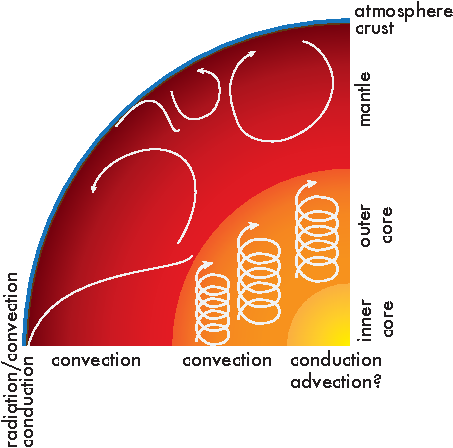
\includegraphics[]{geothermics/figures/earth_heat_mechanisms.pdf}
    \caption{Dominant mechanisms of heat transfer within the Earth.}
    \label{fig:hfmech}
\end{figure}

\subsection{Conduction}
Conduction is the dominant mode of heat transfer in most solid Earth settings relevant to geothermics. It arises from microscopic energy transport by lattice vibrations (phonon--phonon) and, to a lesser extent, free electrons.  Conduction operates in solids and stationary fluids and is the process that underpins essentially all steady-state geotherms and most transient thermal models in the crust and lithosphere.

In this chapter, conduction provides the primary physical link between temperature gradients and observable quantities such as surface heat flow. The diffusion of heat implied by Fourier's law introduces spatial smoothing and finite thermal memory, distinguishing geothermics from purely static potential-field methods.

\subsection{Advection (Convection)}
Advection refers to the transport of heat by the bulk motion of material. In the Earth, this includes mantle convection, magma migration, hydrothermal circulation, tectonic deformation and fluid flow in porous media. While advection can dominate heat transport in many geological environments, it is not treated explicitly as a governing process in many lithospheric thermal studies.

Instead, advective effects are commonly incorporated implicitly through:
\begin{itemize}
    \item boundary conditions---specifically transfer from the convecting mantle to the lithosphere,
    \item effective thermal properties, or
    \item source terms in the energy equation.
\end{itemize}
This approach reflects the focus of geothermics on thermal structure rather than fluid or solid mechanics. Where advection is dominant and explicitly time-dependent, the problem typically shifts into the domain of geodynamics or hydrogeology rather than classical geothermics.

\subsection{Radiation}
Radiative heat transfer involves the emission and absorption of electromagnetic radiation (photons) and governed by the Stefan--Boltzmann law. In the context of the solid Earth, radiative transfer is negligible except at very high temperatures (e.g., in the deep mantle) or at planetary surfaces. Consequently, radiation is not considered further in this chapter.


\section{Conservation of Energy}

The governing equations of geothermics follow directly from the conservation of energy. Consider a representative volume of material in which heat may be conducted ($\vb{q_c}$), advected by material motion ($\vb{q_a}$), radiated ($\vb{q_r}$) or internal sources or sinks ($\vb{q_p}$).  Thus the total vector heat flux out across the surface of a volume, $\vb{q}$, is given by the sum of each mode of transport, i.e.,
\begin{equation}
    \vb{q} = \vb{q_c} + \vb{q_a} + \vb{q_r} + \vb{q_p}.
\end{equation}
The radiative heat flux is generally small at crustal temperatures, but becomes significant at high temperature ($>$\SI{500}{^\circ C}). Often when it is included, it is treated as an enhanced conductive term so requires no special consideration.

In geophysical applications, conduction is described by Fourier's law, a constitutive relation between the conductive heat flux and the temperature gradient:
\begin{equation}
    \coreeq
    \vb{q_c} = k \, \grad{T},
    \label{eq:fourier}
\end{equation}
where $k$ is the thermal conductivity, and $T$ is temperature.
\ntextbox{Sign Convention}{
    Because the Earth is losing heat, the heat flow is up away from the surface of the Earth.  By the geophysical definition, this rate of heat loss (heat flow) is defined as positive.  In physics and engineering, the rate of heat loss is typically defined as negative (i.e.\ $q = - k \grad T$).
}{alert}
Advection results in additional heat flux by the direct transport of mass,
\begin{equation}
    \workeq
    \vb{q_a} = \rho C_P T \vb{u} ,
    \label{eq:advection}
\end{equation}
where $\rho$ is mass density, $C_P$ is specific heat capacity at constant pressure, $\vb{u}$ is the material or fluid velocity, and $T$ is temperature. We will often see coupled $\rho C_P$ in geothermics which is collectively known as the heat storage capacity or simply heat capacity.

In Earth, there are a number of potential sources and sinks of heat.  The most important and continuous source is due to radioactive decay.  Shear heating from deformation in shear zones, bending and folding, and slipping on faults all produces frictional heat.  This heating while important locally can add to regional heat flow over geologic time (Box~\ref{box:shearheat}).  Phase changes during melting and metamorphism can act as both a source (crystallization/retrograde) or sink (melting/prograde) of heat.  Although they can be written as an effective source term in the energy equation, their magnitude is controlled by the rate of reaction progress along a $P$--$T$ path, making them time dependent and fundamentally different from volumetric heat sources such as radiogenic and shear heating.  Melting and metamorphism are discussed further in Section~\ref{sec:stefan}.  Since radioactive heat generation dominates, we'll focus on this component of the internal heat flux, which is expressed as
\begin{equation}
    \workeq
    \vb{q_p} = A \vb{x}
    \label{eq:qsources}
\end{equation}
where $A$ is the heat production per unit volume.

\ntextbox{Shear heating in the Earth}{
    Deformation of a viscous material converts mechanical work into heat, a process known as \emph{shear heating} (or viscous dissipation).  In its most general form, the volumetric heating rate depends on the stress and the full velocity gradient.  However, for most geophysical applications, this expression can be simplified by working in terms of a characteristic strain rate.

    For a viscous material with effective viscosity $\eta$ and second invariant of the strain rate tensor $\dot{\varepsilon}$, the shear heating rate can be approximated as
    \[
        \Phi \approx \eta\,\dot{\varepsilon}^2,
    \]
    where $\Phi$ has units of \si{W.m^{-3}}.  This expression highlights two important features. First, shear heating is always positive, representing irreversible conversion of mechanical energy into heat.  Second, the heating rate scales with the square of the strain rate, so even modest increases in deformation rate can lead to large increases in heating.

    To assess the importance of shear heating, we can compare it with typical radiogenic heat production in the mantle, which is approximately $2 \times 10^{-8}~\si{W.m^{-3}}$

    Using representative mantle values ($\eta \sim 10^{21}$~\si{Pa.s}, $\dot{\varepsilon} \sim 10^{-15}~\si{s^{-1}}$), we find $\Phi \approx 10^{-9}~\si{W.m^{-3}}$.  This result is only a few percent of the radiogenic contribution.  Thus, in the convecting mantle interior, shear heating is typically negligible.  However, because $\Phi \propto \dot{\varepsilon}^2$, shear heating increases rapidly in regions where deformation is localized.  In lithospheric shear zones or subduction interfaces, strain rates can be orders of magnitude higher, and shear heating may become comparable to or exceed radiogenic heating.

    Strain rates in tectonic environments span many orders of magnitude (Table~\ref{tab:strainrates}), primarily reflecting differences in the spatial scale over which deformation occurs.
    \begin{center}
    \textbf{Table~\thetable:} Typical strain rates in tectonic settings and their implications for shear heating.
    \label{tab:strainrates}
    \begin{tabular}{lccc}
    \toprule
    \textbf{Setting} &
    \textbf{Strain rate}  &
    \textbf{Shear heat production} &
    \textbf{Importance} \\
    & (\si{s^{-1}}) & \si{W.m^{-3}} \\
    \midrule
    Mantle interior & $10^{-16}$--$10^{-15}$ & $10^{-11}$--$10^{-9}$ & negligible \\
    Mid-ocean ridges & $10^{-15}$--$10^{-14}$ & $10^{-9}$--$10^{-7}$ & small \\
    Subduction zones & $10^{-14}$--$10^{-13}$ & $10^{-7}$--$10^{-5}$ & moderate \\
    Lithospheric shear zones & $10^{-13}$--$10^{-12}$ & $10^{-5}$--$10^{-3}$ & important \\
    Earthquakes & $10^{-6}$--$10^{2}$ & $10^{1}$--$10^{9}$ and higher & extreme (transient) \\
    \bottomrule
    \end{tabular}
\end{center}

    Although shear heating is typically small in the well-mixed mantle interior, it can play an important role in localized regions of high strain.  In such settings, the strong dependence on strain rate can lead to thermal weakening, potentially promoting further localization of deformation.  This feedback is thought to be important in the development of plate boundaries and ductile shear zones.

    In tectonic environments, deformation is commonly concentrated into narrow zones such as faults and shear zones, so that high strain rates—and therefore significant shear heating—are restricted to relatively small volumes of the lithosphere.  As a result, while temperatures within these zones may locally increase substantially, in some cases even approaching melting conditions, the integrated effect on the thermal structure of the lithosphere as a whole is much smaller.

    In the crust, the presence of fluids along faults can further moderate the thermal impact of shear heating.  Fluid circulation enhances heat transport away from deforming zones, allowing heat to be dissipated more efficiently and reducing the magnitude and duration of local temperature increases.
}{aside}\label{box:shearheat}

Conservation of energy requires that the rate of change of internal energy equal the divergence of heat flux plus any internal heat sources.  In differential form, the general statement relevant to geothermics can be written as
\begin{equation}
    \pdv{(\rho C_P T)}{t} = \div{\vb{q}}.
\end{equation}
Writing energy conservation with the storage term form makes it explicit that density and heat capacity may vary with temperature.  Substituting Equations~\ref{eq:fourier}, \ref{eq:advection} and~\ref{eq:qsources} into the above, yields the advection--diffusion equation for heat:
\begin{equation}
    \coreeq
    \mlbox[
        labelstyle={xshift=-3em,yshift=-7em},
        linestyle={out=90,in=270, latex-}]
    {\pdv{(\rho C_P T)}{t}}{transient} =
    \mlbox[
        labelstyle={xshift=-3em,yshift=1em},
        linestyle={out=270,in=90, latex-}]
    {\div (k \grad T)}{diffusion} - 
    \mlbox[
        labelstyle={xshift=-3em,yshift=1em},
        linestyle={out=270,in=90, latex-}]
    {\div (\rho C_P \vb{u} T)}{advection} + 
    \mlbox[
        labelstyle={xshift=3em,yshift=-6em},
        linestyle={out=90,in=270, latex-}]
    {A}{sources},
  \label{eq:heateq}
\end{equation}
This equation is parabolic in time and describes the combined effects of thermal storage, diffusion, advective transport, and internal heat production. It forms the fundamental basis for both steady-state and transient thermal models, with different terms dominating in different geological environments.

In this text, we will generally ignore situations involving advection.  We will make additional simplifying assumptions to solve special cases consistent with tectonic scenarios.

\subsection{Steady-State and Conductive Limit}
In the absence of advection ($\vb{u}=0$) and when thermal conditions ($\pdv{T}{t} \approx 0$) do not change appreciably with time, the conservation-of-energy equation reduces to
\begin{equation}
    \coreeq
    \div (k \, \grad{T}) = -A.
\end{equation}
This elliptic equation governs steady-state conductive geotherms and places geothermics on the same mathematical footing as gravity, magnetics, and electrostatics, while retaining explicit dependence on material properties and internal heat sources.  This equation shows that the curvature of the temperature field is controlled directly by internal heat production and spatial variations in thermal conductivity.

\subsection{Interpretation}
The conservation-of-energy framework highlights three central features of geothermics:
\begin{enumerate}
    \item temperature is a state variable with finite storage capacity ($\rho C_P$),
    \item thermal structure reflects both present-day boundary conditions and the integrated effects of past processes, and
    \item departures from purely conductive behavior arise through advection and property variations rather than changes in the governing physical principle.
\end{enumerate}
These properties distinguish geothermics from static potential-field methods and motivate the explicit consideration of timescales, transients, material properties, and thermal memory throughout this chapter.

\ntextbox{The heat equation as a configurable system}{
    The heat equation (Equation~\ref{eq:heateq}) can be thought of as a configurable system, much like purchasing a car.

    At its simplest, one can choose the base model: no options, no add-ons, and no complexity. In geothermics, this corresponds to Laplace's equation, where there are no internal heat sources, no time dependence, and nothing moving (hopefully the base car moves). The problem is elegant, tractable, and often admits analytic solutions.

    Adding internal heat production is like selecting an upgraded engine. The governing equation becomes Poisson's equation, and while the physics becomes more realistic, the solution space becomes more complex. Curvature appears, and interpretation requires additional information.

    Including time dependence introduces another major upgrade. The full diffusion equation describes how temperature evolves, retains memory of past conditions, and responds on characteristic timescales set by thermal diffusivity. Many previously simple problems now require numerical solutions.

    Additional features—such as advection, latent heat, moving boundaries, or variable material properties—each add capability but also cost. The governing equation remains the same in principle, but solutions become progressively harder to obtain and harder to interpret.

    Just as with a car, the question is not whether one should always choose the most fully equipped option, but which configuration is appropriate for the problem at hand.
}{aside}


\section{Thermal Properties of Earth Materials}
This is where geothermics really differentiates itself from gravity and magnetics.

This section develops the thermal properties that control conductive and transient heat transport in the lithosphere, with emphasis on thermal conductivity and radiogenic heat production. The goal is not to present canonical constants, but to show how these properties vary systematically with lithology, composition, temperature, pressure, metamorphic grade, and tectonic setting, and how those variations influence geothermics and interpretation. Rather than treating thermal properties as fixed parameters, they are presented here as spatially variable fields whose structure reflects geological history.

The treatment leans on recent syntheses and global compilations, particularly for continental crustal rocks, which have substantially revised earlier assumptions about uniformity and simple depth dependence of thermal properties.


\subsection{Thermal Conductivity, $k$}
\subsubsection{Functional Role of Conductivity}
Thermal conductivity, $k$, controls how efficiently heat is redistributed by conduction and therefore governs both the shape of geotherms and the attenuation of lateral thermal variations. In most crustal rocks, heat is transported primarily by lattice vibrations (phonons), with a smaller contribution from free electrons that becomes significant only in metallic or graphitic materials. The efficiency of this transport is reduced by scattering from defects, grain boundaries, and interfaces between mineral phases, so that conductivity depends sensitively on mineralogy, microstructure, and fabric.

A central point for geothermics is that thermal conductivity redistributes heat but does not generate it. As a result, conductivity primarily controls temperature gradients and the smoothing of thermal structure, rather than the absolute thermal budget. Variations in $k$ therefore influence how heat is expressed spatially, not how much heat is available.

Thermal conductivity is not constant, even within a single lithology. In crystalline rocks it generally decreases with increasing temperature, reflecting enhanced phonon scattering at higher vibrational energies. Pressure effects are typically weaker but become non-negligible at lower crustal conditions. Together, these dependencies introduce nonlinearity into both steady-state and transient thermal models when large temperature ranges are involved, and motivate the use of temperature-dependent conductivity in lithospheric studies rather than constant values. Recent work has emphasized that neglecting this dependence can lead to systematic biases in inferred geotherms, particularly in the lower crust and lithosphere.

In many geological settings, thermal conductivity is anisotropic. Foliation, layering, and mineral alignment can cause heat to flow more readily in some directions than others. Even when anisotropy is modest, spatial variations in $k$ lead to thermal refraction, in which heat flow is redirected across lithological boundaries. This effect is directly analogous to refraction in other potential fields and can significantly alter local geothermal gradients without changing the total heat flux.

\subsubsection{Compositional Variations}

Conductivity varies systematically with lithology and composition. These differences matter in geothermics not because they change how much heat is generated, but because they control how efficiently heat is redistributed through the crust.  Felsic rocks tend to exhibit lower conductivities than mafic rocks (Figure~\ref{fig:tc_rock_type}), while quartz content exerts a first-order control in many common crustal lithologies. Metamorphic recrystallization can further modify conductivity through grain growth, phase changes, and the destruction or enhancement of preferred mineral alignments. Global datasets demonstrate that these lithology-dependent variations are large enough to matter for regional and continental-scale geotherms, especially in the upper crust where lateral heterogeneity is greatest.
\begin{figure}
    \centering
    
\includegraphics[width=14cm]{geothermics/figures/conductivity_distributions.pdf}
    \caption{Thermal conductivity of common igneous and metaigneous and a few metasedimentary rock types.  Rock types have been recomputed based on chemistry for consistent naming.  The rock types are ordered vertically with \ce{SiO2} from highest at the top to lowest at the bottom.}
    \label{fig:tc_rock_type}
\end{figure}


Unlike heat production, which can be highly variable for any given rock type, thermal conductivity is easier to estimate.  A number of mixing laws have been used to estimate thermal conductivity either of a rock with varying porosity, or as an assemblage of minerals.  The most common mixing relation used to estimate the effective thermal conductivity is the geometric mean:
\begin{equation}
    k_{\mathrm{eff}} = \prod_{i=1}^{N} k_{i}^{\chi_{i}},\;
    i = 1, 2, \ldots N,
\end{equation}
where $\chi_{i}$ is the volume fraction of the constituent minerals and/or pore filling components.  Note: the notation denoted by,$\prod$, indicates a product analogous to $\sum$, e.g., $\prod_{i=1}^N a_i^2 = a_1^2 a_2^2 a_3^2 \cdots a_N^2$. The geometric mean as a mixing model works best for rocks where the minerals are randomly arranged and oriented and so works best for fresh igneous rocks. The thermal conductivity of several common minerals are listed in Table~\ref{tab:tcmin}.
\begin{table}[bpht]
    \centering
    \begin{threeparttable}
    \caption{Thermal conductivity of common materials.}
    \label{tab:tcmin}
    \begin{tabular}{lc}
        \toprule
        {} &
        $k$ \\
        mineral &
        W m$^{-1}$K$^{-1}$ \\
        \midrule
        air               & 0.026  \\
        water             & 0.6    \\
        ice               & 2.5 (@ -30\degC) \\
        oil               & 0.13   \\
        salt (halite, sylvite) & 6, 7 \\
        iron              & 80 \\
        copper            & 401 \\
        calcite           & 3.6   \\
        $\alpha$-quartz   & 8.8   \\
        orthoclase        & 1.8   \\
        plagioclase, felsic (Ab$_{80}$An$_{20}$) & 1.8 \\
        plagioclase, mafic (Ab$_{35}$An$_{65}$) & 1.6 \\
        mica, muscovite ($\parallel$,$\perp$)   &  3.9, 0.6  \\
        mica, biotite ($\parallel$,$\perp$)     &  3.1, 0.5  \\
        hornblende        &  2.7  \\
        clinopyroxene (Di$_{90}$Hd$_{10}$)    &  4.3  \\
        orthopyroxene (En$_{90}$Fs$_{10}$)     &  3.4  \\
        olivine (Fo$_{90}$) &  4.8  \\
        spinel (Sp$_{75}$Mt$_{25}$) & 9? \\
        garnet (Py$_{70}$Al$_{30}$)       &  3.9 \\
        \bottomrule
    \end{tabular}
    \begin{tablenotes}
        \item All conductivities estimated at \SI{25}{\degC}.
    \end{tablenotes}
    \end{threeparttable}
\end{table}
 % tab:tcmin

For silicate rocks and clastic sediments, the dominant control on the thermal conductivity is the quartz content as it has a thermal conductivity significantly higher than most other common minerals.  For sedimentary rocks the porosity is also very important.

Like most physical properties of rocks, thermal conductivity is sensitive to pressure and temperature effects.  Thermal conductivity typically decreases with temperature while pressure tends to slightly increase the thermal conductivity slightly.  The thermal conductivity of most rocks tend to about \SI{2.5}{\tcu}\ at high temperatures regardless of their mineralogy.  An example is shown for olivine in Figure~\ref{fig-kol}.
\begin{figure}[hbtp]
  \centering
  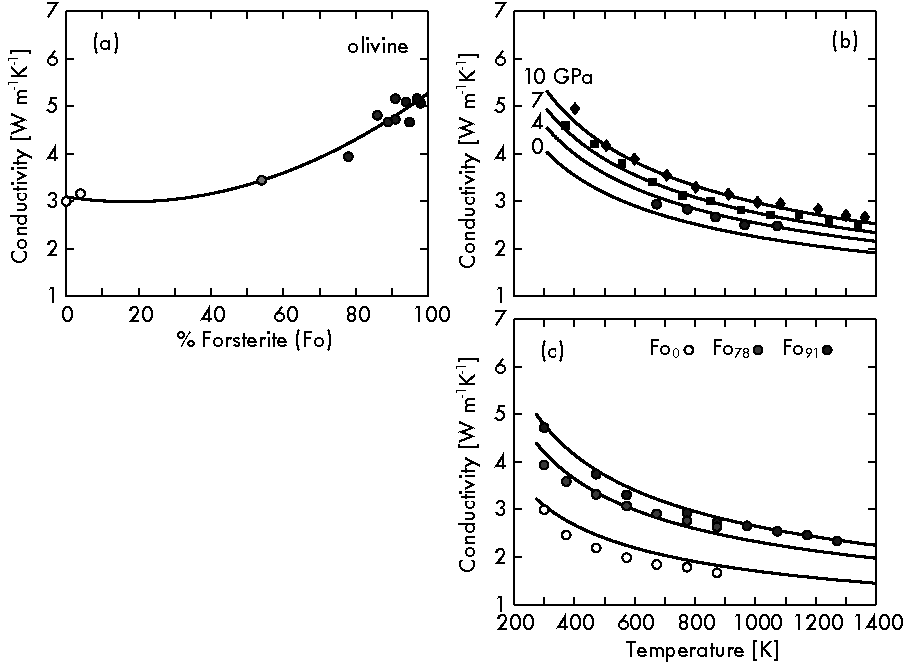
\includegraphics{geothermics/figures/k_olivine.pdf}
  \caption{Thermal conductivity of olivine. (a) Compositional dependence at
  \SI{298}{K}. (b) Pressure and temperature dependence. (c) Compositional and
  temperature dependence.}
  \label{fig-kol}
\end{figure}

At higher temperatures, generally $>\SI{500}{\degC}$, thermal conductivity is enhanced by radiative transmission.  At high temperatures, some minerals are transparent, allowing photons to transfer energy at a greater distance through the crystal until they interact with the lattice (photon-phonon transmission).  However, the radiative effect for many minerals is still poorly constrained. Recent experiments on olivine suggest the influence is nearly double what was previously believed \citep{Marzotto_etal2025}.

\subsection{Anisotropy}
Thermal conductivity is an anisotropic property, meaning that its magnitude depends on the orientation along which it is measured.  Anisotropy can arise at micro-, meso-, and macroscopic scales.  Macroscopic anisotropy, discussed further in Section~\ref{sec:thermresist}, reflects large-scale heterogeneities such as stratified lithologies or laterally continuous compositional layers.  Mesoscopic anisotropy operates at the scale of hand samples or outcrops and is the focus of this section.

Mesoscopic anisotropy may result from compositional layering, preferred orientation of intrinsically anisotropic minerals, or a combination of both.  At this scale, anisotropy commonly develops during deformation, where shearing and compaction produce foliation or lineation that aligns mineral grains and pores.  This alignment creates a plane of approximately uniform thermal conductivity, with a perpendicular direction that exhibits a distinct value.

Many common rock-forming minerals exhibit crystallographic anisotropy in thermal conductivity, including quartz, feldspar, pyroxene, and olivine.  In contrast, garnet is one of the few major rock-forming minerals that is effectively isotropic due to its isometric crystal structure.  Consequently, bulk-rock anisotropy is strongly controlled by both mineral assemblage and fabric, rather than by composition alone.

Anisotropy is typically quantified by measuring thermal conductivity along multiple orientations relative to foliation or lineation (Figure~\ref{fig:tc_anisotropy}).  For samples with transverse isotropy, an anisotropy factor can be defined as
\[
    \workeq
    \Lambda = \frac{\max(k_\parallel,k_\perp)}{\min(k_\parallel,k_\perp)},
\]
where $k_\parallel$ and $k_\perp$ denote conductivities measured parallel and perpendicular to the foliation plane, respectively.
\begin{figure}[tbh]
    \centering
    
\includegraphics[]{physprop/figures/observed_anisotropy_angle.eps}
    \caption{Directional dependence of thermal conductivity measured relative to fabric orientation in an anisotropic metasedimentary samples. Conductivity measured parallel to layering or mineral alignment differs systematically from measurements made perpendicular to layering.}
    \label{fig:tc_anisotropy}
\end{figure}

Among sedimentary and metasedimentary rocks, both isotropic and anisotropic behaviors are observed.  Anisotropy cannot be predicted uniquely from bulk composition alone, as it depends on the degree of fabric development and mineral alignment.  However, certain compositions are more prone to anisotropy than others.  In particular, rocks with bulk compositions near \SI{65}{wt\%} \ce{SiO2} commonly exhibit elevated anisotropy factors (Figure~\ref{fig:k_aniso}), coinciding with peak abundances of sheet silicates.  These minerals possess strong intrinsic anisotropy and readily align during deformation, amplifying bulk thermal conductivity contrasts.
\begin{figure}[hbtp]
    \centering
    \includegraphics[]{geothermics/figures/k_anisotropy_oxides.eps}
    \caption{Anisotropy factor variations with \ce{SiO2} and \ce{K2O}.  While there is not a single function to describe the data, the envelope of permissible anisotropy factors varies with composition.}
    \label{fig:k_aniso}
\end{figure}
%- Lithology variations
% Add a figure like the heat production for thermal conductivity
%- Anisotropy
% Add a figure with thermal conductivity anisotropy and SiO2, repeat of figure from the physical properties chapter.

\subsection{Radiogenic Heat Production, $A$}

\section{Heat Production, $A$}

Radiogenic heat production, $A$, supplies internal energy to the crust and is the primary control on the curvature of continental geotherms. In contrast to thermal conductivity, which redistributes heat without creating or destroying energy, heat production acts as a true volumetric source term in the heat equation. As a result, it governs how temperature departs from linearity with depth and exerts first-order control on crustal thermal structure.

At present day, crustal heat production is overwhelmingly dominated by the radioactive decay of potassium, thorium, and uranium, which together account for $\gtrapprox 99\%$ of radiogenic heat generation. Minor contributions arise from rubidium and samarium  (Table~\ref{tab:radiostopes}). Numerous other naturally occurring radioisotopes exist, but their present-day contribution to Earth''s heat budget is negligible.

Heat production is not constant through geological time because radioactive decay reduces the abundance of key isotopes (Box~\ref{box:hp_time}). This process is monotonically decreasing with age. Reconstructing past geotherms therefore requires accounting for the time evolution of isotope abundances and the resulting change in heat production.
\begin{table}
    \centering
    \begin{threeparttable}
    \caption{A table of radiogenic isotopes relevant to Earth's heat production \citep{McDonough_etal2020}.}
    \label{tab:radisotopes}
    \begin{tabular}{@{}ccccc@{}}
        \toprule
        \textbf{Isotope} &
        \textbf{Half-life} &
        \textbf{Decay Constant} &
        \textbf{Abundance}\tnote{a} &
        \textbf{Heat Generation} \\
        & \si{Ma} & \si{a^{-1}} & \% & \si{\mu W.kg^{-1}} \\
        \midrule
        \ce{^{26}Al}  & \SI{0.717(24)}{ka} & $9.67 \times 10^{-7}$    & 0        & $3.41 \times 10^5$ \\
        \ce{^{40}K}   & $1.262(2)$    & $5.491 \times 10^{-10}$  & $1.167 \times 10^{-4}$ & 29.029 \\
        \ce{^{60}Fe}  & \SI{2.62(4)}{ka}  & $2.65 \times 10^{-7}$    & 0        & $3.99 \times 10^4$ \\
        \ce{^{87}Rb}  & $49.61(16)$   & $1.397 \times 10^{-11}$  & 0.2783   & 0.04082 \\
        \ce{^{147}Sm} & $106.3(5)$    & $6.539 \times 10^{-12}$  & 0.14993  & 0.3073 \\
        \ce{^{232}Th} & $14.1(1)$     & $4.92 \times 10^{-11}$   & 1.0000   & 26.180 \\
        \ce{^{235}U}  & $0.70348(20)$ & $9.8531 \times 10^{-10}$ & 31.223   & 561.65 \\
        \ce{^{238}U}  & $4.4683(96)$  & $1.5513 \times 10^{-10}$ & 0.992740 & 94.936 \\
        \bottomrule
        \addlinespace[0.6em]
    \end{tabular}
    \begin{tablenotes}
        \item[a]Short lived isotopes \ce{^{26}Al} and \ce{^{60}Fe} are negligible today, but would have been important contributors to the heat production in the early Earth.
    \end{tablenotes}
    \end{threeparttable}
\end{table}

If we go back in time to the formation of Earth, two short-lived radionuclides---\ce{^{26}Al} and \ce{^{60}Fe}---played a major role during Earth's earliest evolution. During the first $\lesssim$20~Ma of planetary history, decay of these isotopes generated nearly \SI{1000}{TW} of heat, profoundly influencing early melting and differentiation. Although their abundances are now negligible, some of this early thermal energy continues to be lost from Earth's interior. By comparison, radiogenic heat production today is approximately \SI{20}{TW}. Relevant radiogenic isotopes and their properties are summarized in Table~\ref{tab:radisotopes}.

\subsection{Quantifying Heat Production}

Present-day heat production can be computed directly from bulk chemical compositions using
\begin{equation}
    \workeq
    A~[\hgu] = \rho \left(3.387 \times 10^{-3}\,\ce{K} + 26.18\,\ce{Th} + 98.29\,\ce{U} + 0.01139\,\ce{Rb} + 0.04595\,\ce{Sm}\right),
\end{equation}
where elemental concentrations are given in weight percent and $\rho$ is density. Because uranium and thorium have much higher heat productivity per unit mass than potassium, small variations in trace-element abundance can dominate $A$ even when K varies substantially.

Heat-producing elements are not uniformly distributed among rock-forming minerals. Instead, they are preferentially concentrated in accessory phases such as zircon, monazite, xenotime, allanite, apatite, and related phosphates. Consequently, radiogenic heat production is highly sensitive to magmatic differentiation, partial melting, sedimentary recycling, and other crustal processing mechanisms. This leads to variations in $A$ spanning several orders of magnitude among lithologies (Figure~\ref{fig:hp_rtype}), even within a single tectonic province.
\begin{figure}[htp]
    \centering
    \includegraphics[]{geothermics/figures/hp_rtype.eps}
    \caption{Heat production of (a) plutonic (igneous) and (b) sedimentary rock types determined from a global geochemical database \citep{Hasterok_etal2017}.  Inset diagrams display the chemical divisions used to define the igneous and sedimentary rock types, respectively.}
\end{figure}

\subsection{Geological Controls on Heat Production}

Potassium behaves as a major element and is abundant in feldspars, micas, clays, and some amphiboles, all common constituents of the upper crust. Uranium and thorium, by contrast, are trace elements and are typically hosted in dense accessory minerals, particularly monazite-group phosphates. These minerals may be mechanically concentrated during weathering and sedimentary sorting, allowing heat-producing elements to become enriched in specific depositional environments (Figure~\ref{fig:hpe}).

All major heat-producing elements are incompatible during partial melting. Melting therefore preferentially extracts K, Th, and U from the source rock and transports them toward the surface, where they are further concentrated by fractional crystallization or sedimentary reworking (Figure~\ref{fig:hpe}). In addition, uranium is mobile in oxidizing fluids and may be redistributed by groundwater, leading to enrichment in mudstones, shales, and other fine-grained sedimentary rocks.
\begin{figure}[htbp]
    \centering
    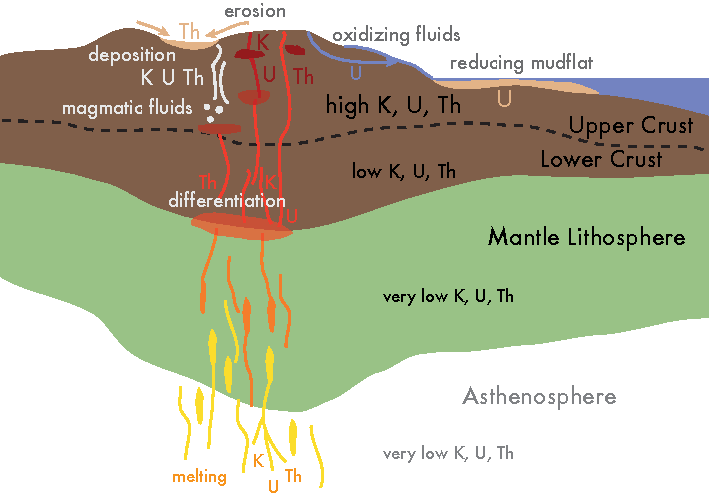
\includegraphics[]{geothermics/figures/hpe_dynamics.pdf}
    \caption{Dynamics of heat producing elements and their path from the mantle
    to concentrations within the crust.}
    \label{fig:hpe}
\end{figure}

Systematic differences in heat production are observed across tectonic settings. Felsic and intermediate compositions generally exhibit higher heat production than mafic rocks, while cratons, mobile belts, arcs, and sedimentary basins occupy distinct characteristic ranges.

There is a prevailing view that metamorphic grade and repeated crustal reworking can further redistribute heat-producing elements, modifying thermal structure over time.  Early studies of heat production were interpreted as a decreasing heat production with increasing metamorphic grade. The datasets that these were based on were small, not based on individual lithologies, and produced mixed results.  More recent studies, including several high-resolution surveys by \citet{Alessio_etal2018} suggest that heat production is not affected.  More work is needed, but be careful accepting old wisdom before you know where it comes from.

Heat production varies with igneous crystallization age. For much of the past \SI{2.0}{Ga}, heat production in igneous rocks occupies a relatively narrow range, while older crust shows a systematic decrease in $A$ with increasing age (Figure~\ref{fig:hp_age}). Because mid-ocean ridge basalts derive from strongly depleted mantle sources, their heat production is substantially lower than that of continental lithosphere. Typical values for major lithospheric reservoirs are summarized in Table~\ref{tab:hpe}.
\begin{figure}[hbtp]
    \centering
    \includegraphics[]{geothermics/figures/hp_v_age.eps}
    \caption{Heat production variations with age for several igneous rock compositions \citep{Gard_etal2019a}.}
    \label{fig:hp_age}
\end{figure}
\begin{table}[hbtp]
    \centering
    \caption{Heat production averages.}
    \label{tab:hpe}
    \begin{tabular}{lc}
        \toprule
        {} & \textbf{Heat Production} \\
        \textbf{Reservoir} & \hgu \\
        \midrule
        \multicolumn{2}{c}{\it continental} \\
        upper crust &   2 \\
        lower crust &   0.4 \\
        mantle lithosphere &    0.02 \\
        \multicolumn{2}{c}{\it oceanic} \\
        crust, altered (unaltered) & 0.07 (0.3) \\
        mantle lithosphere & 0.002 \\
        \bottomrule
    \end{tabular}
\end{table}

Recent studies reveal systematic relationships between radiogenic heat production, magmatic differentiation, and crustal thickness in arc systems (Figure~\ref{fig:hp_arcs}). Although the underlying mechanisms are not yet fully understood, similar trends are observed for many trace elements, suggesting that heat production is part of a broader geochemical signal associated with crustal growth. These relationships link geothermics with petrology and tectonics, highlighting thermal properties as valuable tracers of crustal evolution.
\begin{figure}[htbp]
    \centering
    \includegraphics[]{geothermics/figures/hp_v_moho.eps}
    \caption{Heat production in recent arc volcanics and their relationship to crustal thickness.  The three arcs circled in grey are excluded from the analysis as their heat production is anomalous, likely resulting from the recent subduction of continental crust and/or thick continental derived sediments (\emph{Hasterok unpublished}).}
    \label{fig:hp_arcs}
\end{figure}

Two key conclusions follow. First, heat production is generally highest in the upper crust, lower in the lower crust, and lowest in the mantle. Second, the natural variability of heat production is sufficiently large that reliable estimates require direct observation---either geochemical analysis or gamma-ray spectrometry---rather than inference alone.

\subsection{Depth Distributions and Modeling Assumptions}

Constraints on how heat production varies with depth in the crust remain incomplete and, in some cases, contradictory. From a thermal modeling perspective, one requirement is clear: if surface-measured heat production is extended to excessive depths, conductive geotherms fail to intersect the mantle adiabat. This fundamental constraint implies that heat production must decrease downward on average, but it does not uniquely determine how that decrease is achieved.

Geological and geophysical observations provide competing lines of evidence. Seismic velocity models and bulk chemical arguments suggest that the crust becomes progressively more mafic with depth, which would imply a systematic reduction in heat production due to lithologic control. However, even when surface heat production values appropriate for mafic compositions are extended downward, model geotherms commonly remain too warm. Direct observations from lower-crustal xenoliths are broadly consistent with reduced heat production, but these samples are drawn from a limited number of terranes and may be biased toward Archean crust, which is itself characterized by relatively low heat production.

At the same time, some recent models of crustal composition argue that the lower crust may be more felsic than traditionally assumed. Granulite-facies felsic rocks can exhibit densities and seismic velocities comparable to those of lower-crustal mafic rocks, complicating purely seismic interpretations. If such compositions are widespread, they would imply higher heat production at depth than standard mafic models suggest. Nevertheless, surface heat production observations still require that average lower-crustal values be lower than those inferred from exposed upper-crustal rocks, even if the precise magnitude and cause of the decrease remain uncertain.

To represent this downward reduction in heat production, many thermal models adopt an exponential decay of heat production with depth. This parameterization is computationally convenient but lacks a physical basis, and should not be interpreted as a process-based description. Global geochemical compilations reveal large variability in heat production among terranes of similar thickness and structure, indicating that depth distributions are not governed by simple physical rules. Instead, they emerge from the cumulative effects of magmatism, sedimentation, metamorphism, and tectonic accretion through time.

These observations emphasize that heat production is geologically structured rather than smoothly varying with depth. Its distribution reflects crustal assembly history as much as present-day lithology. As a consequence, assumptions about $A(z)$ represent one of the dominant sources of uncertainty in crustal geotherm modeling, and simple parameterizations should be treated as pragmatic approximations rather than physically meaningful descriptions.

\subsection{Modeling Consequences}

Thermal conductivity and heat production jointly determine the shape of geotherms. Heat production primarily controls curvature, while conductivity governs the magnitude of temperature gradients (temperature--depth slope) and the redistribution of heat. Because different combinations of $k$ and $A$ can yield similar temperature-depth profiles, trade-offs between these parameters are a major source of non-uniqueness in thermal models. Robust interpretation therefore requires independent geological or geophysical constraints on both properties.

Several general implications follow for geothermics. Thermal properties should be treated as spatially variable fields rather than fixed constants, particularly in the upper crust where lateral heterogeneity is pronounced. Variations in conductivity and heat production can produce substantial differences in local geotherms even when surface heat flow is similar. Simple parameterizations may reproduce average behavior but often fail to capture observed variability, underscoring the importance of geological constraints, temperature-dependent properties, and sensitivity analysis in both steady-state and transient models.

\ntextbox{Time Dependence of Radiogenic Heat Production}{
    Radiogenic heat production decreases with time as radioactive isotopes decay. Reconstructing geotherms in the geological past therefore requires explicit accounting for the time evolution of isotope abundances and their heat production. The expressions below provide a framework for computing past heat production directly from present-day rock compositions and are intended for use in forward thermal modeling exercises.

    The heat production contribution from a single isotope, $i$, from element, $j$, is given by
    \[
        A_{i,j} = \rho H_{i,j} C_{i,j} ,
    \]
    where $\rho$ is the rock density, $H_i,j$ is the heat production per unit mass and $C_i,j$ is the mass fraction (\si{kg}/\si{kg}) of the isotope.  Since we typically measure the concentration of elements rather than isotopes in a rock, we can write the heat production contribution as
    \[
        A_{i,j} = \rho H_{i,j} X_{i,j} C_j
    \]
    where $X_{i,j}$ is the aboundance of isotope $i$ in element $j$.

    For the radioactive isotope, $X_{i,j}$, the number of atoms decreases exponentially with time.  Turning the equation around to solve for the heat produced in the past,
    \begin{equation}
        \workeq
        X_{i,j}(t) = X_{i,j,0}\,e^{\lambda_i t},
    \end{equation}
    where $\lambda_i$ is the decay constant for isotope $i$, and $t$ is time defined as positive moving into the geological past.

    The total volumetric heat production at time $t$ is then
    \[
        \workeq
        A(t) = \rho \sum_i \sum_j H_{i,j} X_{i,j,0} C_{j} \,e^{+\lambda_i t},
    \]
    with the summation taken over all heat-producing isotopes and $\rho$ the rock density. Note that this formulation assumes closed-system behavior and constant bulk composition through time.

    For practical applications involving crustal rocks younger than approximately \SI{4}{Ga}, the dominant contributions come from \ce{^{238}U}, \ce{^{235}U}, \ce{^{232}Th}, and \ce{^{40}K}. Because \ce{^{235}U} has a much shorter half-life than \ce{^{238}U}, the uranium contribution to ancient heat production increases disproportionately with age, resulting in substantially higher Archean heat production for otherwise identical bulk compositions.

    When coupled with steady-state or transient heat conduction models, these time-dependent heat production terms provide first-order estimates of geotherms throughout Earth history. Even modest increases in $A$ can significantly raise temperatures at depth, highlighting the sensitivity of continental geotherms to the temporal evolution of radiogenic heat sources.
}{core}\label{box:hp_time}

\section{Mantle adiabat and lithospheric thickness}

The conductive lithosphere does not extend indefinitely. Its base is defined by the transition to convecting mantle, whose temperature follows an adiabat (more precisely, an isentrope).

\subsection{Mantle adiabat}
In a convecting fluid with minimial conduction, there is little heat exchanged with the surroundings, resulting in an adiabatic processes (no heat loss). If the process is reversable then it is also isentropic (no entropy loss). The change in pressure during this process is accompanied by a change in temperature.  When temperatures are superadiabtic, material rises, and when they are subadiabatic, the material falls, resulting in convection.

To a reasonable approximation, this describes convection in Earth's mantle, with heat exchanged only at the thermal boundary layers (core--mantle and asthenosphere--lithosphere boundaries.).  It can be shown from the heat equation that this change in temperature with pressure is approximate by
\[
    \left(\frac{\partial T}{\partial P}\right)_S = \frac{\alpha T}{\rho C_P},
\]
where $\alpha$ is the coefficient of thermal expansion, $g$ is gravitational
acceleration, $T$ is temperature, and $C_P$ is the heat capacity at constant
pressure.  This expression can be converted to depth using $dP/dz = \rho g$, giving
\[
    \left(\dv{T}{z}\right)_S \approx \frac{\alpha g T}{C_P}.
\]
The adiabat when projected to the surface reaches what is know as the mantle potential temperature, $T_p$, resulting in a convecting mantle geotherm estimated as
\[
    T_m(z) \approx T_p + z\, \left( \dv{T}{z} \right)_S.
\]
Typical upper-mantle values yield gradients of order 0.3--\SI{0.5}{K.km^{-1}} (Box~\ref{box:adiabat}).

\ntextbox{Estimating the mantle adiabatic gradient}{
    Using the depth formulation for the adiabatic gradient, consider the representative thermophysical properties for fertile upper-mantle garnet lherzolite:
    \begin{align*}
        \alpha &\approx 3\times10^{-5}\,\mathrm{K^{-1}}, \\
        C_P &\approx 1.2\times10^{3}\,\mathrm{J\,kg^{-1}\,K^{-1}}, \\
        T &\approx 1623\,\mathrm{K}, \\
        g &= 9.8\,\mathrm{m\,s^{-2}}.
    \end{align*}

    Substituting these values gives
    \[
        \left( \dv{T}{z} \right)_S
        \approx
        \frac{(3\times10^{-5})(9.8)(1623)}{1.2\times10^{3}}
        \approx 3.9\times10^{-4}\,\mathrm{K\,m^{-1}}
        \approx 0.39\,\mathrm{K\,km^{-1}}.
    \]

    Over a depth interval of 100~km, the mantle adiabat therefore increases temperature by only $\sim 35$--$\SI{40}{K}$, which is small compared with typical conductive gradients in the lithosphere. This modest slope explains why the lithosphere--asthenosphere boundary is controlled primarily by the conductive geotherm rather than by rapid temperature increase in the convecting mantle.
}{mathtool}\label{box:adiabat}

\subsection{Lithospheric Thickness}

The lithosphere--asthenosphere boundary (LAB) is defined by the transition from a convecting mantle to a conducting lithosphere.  This intersection is defines the depth to the base of the lithosphere, $z = z_L$, i.e., 
\[
    T_{cond}(z_L) = T_m(z_L).
\]
In reality, the transition is not perfectly sharp. Rheological softening, partial melting, and small-scale convection smooth the boundary over tens of kilometers. Nevertheless, the intersection criterion provides a robust and interpretable thermal definition of the lithosphere that links surface observables to mantle conditions.  This thermal definition and may differ from the seismologically defined LAB, which takes a rheological view, though they are often similar in depth.


%----------------------------------------------------------
\section{Steady-State Geotherms}\label{sec:ss}

Steady-state conduction occurs as the long-term asymptotic stabilization of temperature following a transient process. Steady-state geotherms are most applicable to continental geotherms, particularly for those regions which have not experienced tectonic activity in the past few 10's of millions of years. One-dimensional states are sufficiently simple to model analytically, though 2- and 3-D geometries are often sufficiently challenging that they need to be modeled by numerical methods. In this section, we will explore several one-dimensional solutions that are still commonly employed.

\subsection{Homogeneous Lithosphere}

The heat equation as it is written in Equation~\ref{eq:heateq} is very complex; however, we reduce many of the complexities and still reasonably estimate temperatures within the Earth by making reasonable assumptions.
\begin{description}
  \item[Assumption 1:] $\pdv{T}{t} = 0$, i.e., steady-state conditions. \\ This assumption can be risky; however, the time constant for heat transport through a \SI{50}{km} thick lithosphere is approximately \SI{20}{My}.  Rifting in the Basin and Range began in earnest \SI{17}{Ma}, therefore, the lithosphere could be approximated by a near steady-state geotherm.  While this assumption works for many continental regions, it is a poor assumption for evolution of the oceanic lithosphere.

  \item[Assumption 2:] Lateral heat flow is negligible, i.e. $\pdv{T}{x}
  \approx \pdv{T}{y} \approx 0$. \\
  On a large scale, the temperature gradient vertically is approximately two orders of magnitude higher than the lateral gradients, thus the flow of heat is dominated by vertical heat transport.

  \item[Assumption 3:] No advection, i.e., $u = 0$. \\
  While magmatism does bring some heat to the surface, the quantity is too small to be significant for the large scale thermal structure, but can be very important locally (e.g., geothermal areas).

  \item[Assumption 4:] Constant thermophysical properties, e.g.,
  $\pdv{k}{P} = \pdv{k}{T} = 0$. \\
  This assumption is of course not true, but as you will see in Sections~\ref{sec:layeredT} we can work around this complexity by assuming that the properties are constant in sufficiently thin layers.
\end{description}

Making the above assumptions, the heat equation (Equation~\ref{eq:heateq}) is reduced to the differential governing 1-D steady-state heat conduction given by
\begin{equation}
    \dv[2]{T}{z} = -\frac{A}{k}.
    \label{eq-diff}
\end{equation}
To solve this differential equation we need two boundary conditions.  The simplest solution requires surface temperature and heat flow, $T_s$ and $q_{0}$, respectively.  These quantities are possible to measure or estimate relatively easily.  First, we integrate over depth,
\begin{align*}
  \int \dv[2]{T}{z} \dd{z} & = -\int \frac{A}{k} \dd{z}, \\
  \dv{T}{z} & = C_{0} - \frac{A}{k} z,
\end{align*}
giving us the constant $C_{0}$.  At $z = 0$, $\left. \dv{T}{z} \right|_{z=0} = C_{0}$; recalling Fourier's law, $\frac{q_{0}}{k} = C_{0}$.

Integrating a second time, we find:
\begin{align*}
    \int \dv{T}{z} \dd{z} & =
        \int \left( \frac{q_{0}}{k} - \frac{A}{k} z \right) \dd{z} \\
    T & = C_{1} + \frac{q_{0}}{k} z - \frac{A}{2 k} z^{2}.
\end{align*}
Applying the surface boundary condition, $T_{0} = C_{1}$, we arrive at the solution,
\begin{equation}
    \coreeq
    T(z) = T_{0} + \frac{q_{0}}{k} z - \frac{A}{2 k} z^{2}.
    \label{eq:ssgtherm}
\end{equation} 

\subsection{Layered Lithosphere}\label{sec:layeredT}

The homogeneous solution assumes that the thermophysical properties, $k$ and $A$, are constant.  However, thermal conductivity is sensitive to pressure, temperature, and rock type, and heat generation is sensitive to variations in the heat producing elements (U, Th, and K).  All is not lost.  If we make layers thin enough we can assume that the conductivity and heat production are constant with each layer (Figure
\ref{fig:layers}).
\begin{figure}[hbtp]
  \centering
  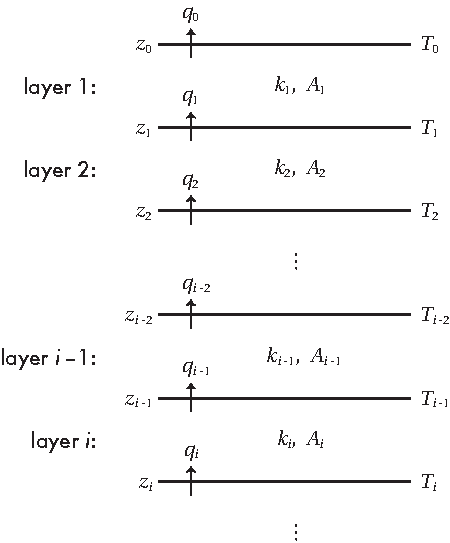
\includegraphics{geothermics/figures/thermal_layers.pdf}
  \caption{Model setup for 1-D steady-state conductive geotherms.}
  \label{fig:layers}
\end{figure}

The solution for the temperature at the base of the first layer, $T_1$, can then be estimated using the homogeneous solution,
\[
    T_1 = T_0 + \frac{q_0}{k_1} (z_1 - z_0) - \frac{A_1}{2 k_1} (z_1 - z_0)^2.
\]
The heat flow at the base of the first layer is equal to
\[
    q_1 = q_0 - A_1 (z_1 - z_0).
\]
The homogeneous solution can then be used to estimate the temperature at the base of the second layer using, $T_1$, as the temperature at the top and $q_1$ as the heat flow.  The temperature of all subsequent layers can be found using the same method boot-strapping down through the domain of interest.  

Solving for the temperature at the base of the $i$-th layer,
\begin{equation}
    \workeq
    T_{i} = T_{i-1} + \frac{q_{i-1}}{k_i} (z_i - z_{i-1})
    - \frac{A_i}{2 k_i} (z_i - z_{i-1})^2.
\end{equation}
It is also necessary to know the heat loss at the base of each layer in order to compute temperature.  Since heat flow is determined by the heat flowing into a layer plus the heat generated within, the heat flow at the bottom of each layer is given by
\begin{equation}
    \workeq
    q_i = q_{i-1} - A_i (z_i - z_{i-1}).
\end{equation}
This solution forms the basis of most 1-D steady-state geotherms.

\ntextbox{Classic Perspective on Geotherms}{
    There are a few classic ideas about how geotherms are constructed that are worth knowing even if their foundational principles are incorrect.  They stem from the historical development of our understanding about heat production and heat flow in the continental lithsphere starting in the 1960's.  The general trends advanced by these models are still reasonable, though ripe for improvement. Though until something better exists, you will still find these widely used. 

    \medskip
    \noindent\textbf{Reduced heat flow}\\
    The concept of reduced heat flow is based around an observed relationship between surface heat flow and surface heat production.  In cases where this relationship occurs, there is a linear correlation between the two sets of observations (higher heat production results in higher heat flow).  Because a linear relationship exists we can fit a linear set of constants to the data, giving,
    \[
        q_s = q_r + A_s D ,
    \]
    where $q_s$ and $A_s$ are the surface heat flow and heat production, respectively.  The intercept of the linear model, $q_r$, is the reduced heat flow and represents the heat flow into the base of an upper crustal layer enriched in heat producing elements.  The slope of the line, $D$, represents the characteristic `thickness' of the enriched layer; however, $D$ only represents the thickness under the constant heat production model (discussed above).

    This relationship is not ubiquitous, but appears to occur under very specific cases in which the plutons that are sampled share a co-genetic relationship (i.e., plutons from the same source and either represent differing degrees of partial melting and/or fractionation).  When all rock types within a geologic province are sampled, the concept of reduced heat flow can quickly break down.  There may be more validity for this relationship where there are regional variations heat flow between geologic provinces in the Canadian Shield.

    \medskip
    \noindent\textbf{Depth Dependent Heat Production}\\
    In the search for heat production models to explain reduced heat flow, three general models were proposed for variations of upper crustal heat production with depth.  These are still in general use today.  Although only the exponential decreasing model preserves the reduced heat flow model for a province under differential erosion.  While each of these models are rarely true in practice, they can be very useful for simplifying the math or as an approximation when knowledge of the system is limited.  The three most common models are:
    \begin{description}
        \item[constant] - a constant heat production with depth is the simplest
        function that one can imagine,
        \[
            A(z) =
            \begin{dcases}
                A_0 & 0 \leq z \leq D \\
                0 & z > D
            \end{dcases}
        \]
        While heat production is never constant with depth, in the absence of any data the constant (or series of constant layers) provides the safest and perhaps easiest approximation to justify for use in computations;

        \item[linear] - since heat production tends to decrease with depth, the simplest ways to model a decrease is as a linear decrease with depth from the surface to some depth ($2D$),
        \[
            A(z) =
            \begin{dcases}
                A_0 \left( 1 - \frac{z}{D} \right) & \text{if } 0 \leq z \leq D \\
                0 & \text{if } z > D
            \end{dcases} .
        \]
        the 2 is necessary to account for a variable of integration, which we will shortly see.  Again, a linear function is quite artificial with little physical justification; and

        \item[exponential] - the exponential decreasing model is meant to solve a problem that arises from the reduced heat flow model (discussed below).  While the other two models are not observed in nature, there are times when an exponential model appears to be roughly observed.  All of the cases where an exponential has been observed (statistically over large scales and with large sample) occur within large, co-genetic batholiths such as the Sierra Nevada Batholith and Idaho Batholith.  The exponential model for upper crustal heat production can be written as
        \[
            A(z) = A_0 e^{-z/D} \quad \text{for } z > 0 ,
        \]
        where $D$ in this case represents the characteristic depth (i.e., depth at
        which $A(D)/A_0 = e^{-1}$).
    \end{description}
    Each of these models provide simple models of upper crustal heat production.  The integration with respect to depth for all three models yields $q_{\mathrm{rad}} = A_0 D$.

    \medskip
    \noindent\textbf{Geotherm families}\\
    The layered steady-state solution can be used to estimate temperatures within the continental crust to great effect (an example of a geotherm is shown in Figure~\ref{fig:kalahari}).  One goal, perhaps, would be to estimate the range of geothermal temperatures one might expect then from typical continental environments.  The best proxy we have for estimating continental temperatures is the surface heat flow.  Regions of high heat flow tend to be warmer than regions of low heat flow.  Therefore, we parameterize our geotherms in terms of surface heat flow.
    \begin{center}
        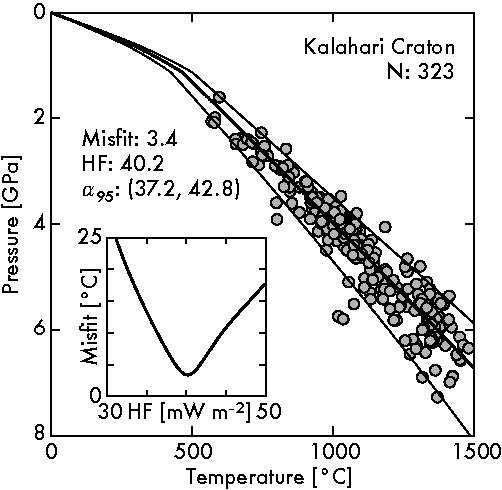
\includegraphics{geothermics/figures/kalahari.pdf}

        \textbf{Figure~\thefigure:} Geotherm for the Kalahari craton calibrated using xenolith $P$--$T$ estimates.
        \label{fig:kalahari}
    \end{center}

    The heat flow at the surface is due to the heat flowing into the base of the lithosphere (the limit of mantle convection) plus any additional heat produced within the lithosphere itself, which we can write,
    \[
        q_0 = q_{\mathrm{LAB}} + q_{\mathrm{sources}}.
    \]
    In general the contributions due to the mantle lithosphere and lower crust are relatively small and their variations have little effect on the geotherm.  Therefore, we can instead view the surface heat flow as the heat flow into the base of an radiogenic enriched layer, $q_{\mathrm{base}}$, and the heat produced within the HPE-enriched surface layer, $q_{\mathrm{uc}}$,
    \[
        q_0 = q_{\mathrm{base}} + q_{\mathrm{uc}}.
    \]

    For regions that have high heat flow, they may have high basal heat flow (input from the mantle), and/or high heat production.  We often assume that the heat production for regions of high heat production are some linear combination of the two, which we can write
    \[
        q_{\mathrm{base}} = P q_0, \quad \mathrm{and} \quad q_{\mathrm{uc}} = (1 - P) q_0,
    \]
    where $P$ is know as the partition coefficient.  From the latter equation, we can estimate the heat production.  We call geotherms parameterized by a single parameter, $P$, in this way a geotherm family.  One such family is shown in Figure~\ref{fig:cont} and provides a reasonable fit to the typical range of temperatures estimated within the continental lithosphere.
    \begin{center}
        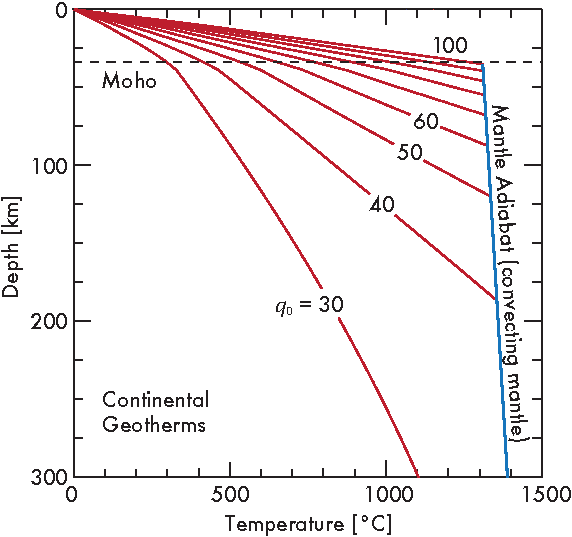
\includegraphics[]{geothermics/figures/continental_geotherms.pdf}

        \textbf{Figure~\thefigure:} A 1-D steady-state geotherm family parameterized in terms of surface heat flow.
        \label{fig:cont}
    \end{center}
}{aside}\label{box:reducedhf}

\subsection{Thermal Resistance}\label{sec:thermresist}
In many basins, the data that are used to estimate heat flow come from bottom hole temperatures (BHTs) in petroleum wells.  These temperatures are notoriously low quality, but with enough data and properly treated, they can give reasonable estimates of heat flow.  Although a basin may have many layers with different thicknesses and thermal conductivities we only need to compute the temperature at the location of the BHT measurement for modeling.  We use the thermal resistance method to compute the temperature at the level of a BHT without having to go through the process of computing the temperature at the base of each layer as outlined above.

To start this derivation, we assume heat generation is negligible, i.e., $A \approx 0$.  For most basins, the effect of heat generation on geothermal temperatures is minimal.  You can test this assumption by choosing a reasonable set of geothermal parameters and computing the heat production to the depth of a deep petroleum well.  Setting $A = 0$ allows us to write the layered model for the $i$-th layer:
\begin{equation}
  T_{i+1} = T_{i} + \frac{q_{i}}{k_{i+1}} (z_{i+1} - z_{i}).
\end{equation}
Since there is no heat generation, the conservation of energy tells us that the heat flowing into the base of each layer must be equivalent to the heat flowing out of the top of each layer.  It follows from this argument that the surface heat flow must be equivalent to the heat flow across each layer, i.e. $q_0 = q_i$ for all $i$.  Since the difference in depths between the bottom and top layer interfaces is the thickness of each layer as we have defined them, we can write the thickness, $h$, as $h_{i+1} = z_{i+1} - z_i$.  Hence, for the first few layers, we can write the temperature at the base of each as
\begin{align*}
    \text{Layer 1:} \quad T_1 &= T_0 + q_0 \frac{h_1}{k_1} , \\
    \text{Layer 2:} \quad T_2 &= T_1 + q_0 \frac{h_2}{k_2} ,  \\
    \text{Layer 3:} \quad T_3 &= T_2 + q_0 \frac{h_3}{k_3} .
\end{align*}
Substituting $T_1$ into the equation for $T_2$ above and then $T_2$ into $T_3$,
we find the temperature at the base of layer three can be written as
\begin{align*}
    T_3 &= \underbrace{
            \underbrace{T_0 + q_0 \frac{h_1}{k_1}}_{T_1}
            + q_0 \frac{h_2}{k_2}
        }_{T_2}
        + q_0 \frac{h_3}{k_3} \\
        &= T_0 + q_0 \left( \frac{h_1}{k_1} + \frac{h_2}{k_2} + \frac{h_3}{k_3}
        \right) \\
        &= T_0 + q_0 \sum_{i=1}^3 \frac{h_i}{k_i} .
\end{align*}
Generalizing the solution for the base of the $i$-th layer,
\begin{equation}
    T_{i} = T_{0} + q_{0} \sum_{i=1}^{N} \frac{h_i}{k_i} .
\end{equation}

This solution now allows us to solve for the temperature at the base of any given layer we wish without having to bootstrap our way from the surface to the depth of interest.  It also leads us to the implication that the effective thermal conductivity of a set of layers is equivalent to the harmonic mean of the conductivities, i.e.,
\begin{equation}
    k_{\mathrm{eff}} = \frac{\sum_{i=1}^N h_i}{\sum_{i=1}^N \frac{h_i}{k_i}} .
\end{equation}

\subsection{Temperatures of a buried sphere}

We have previously solved for the gravity and magnetic field for a buried sphere. In those cases, the sphere is embedded in a uniform background field, and the total field is obtained by superposition of the background and the sphere anomaly. The same principle applies in geothermics. Although the background temperature varies with depth, it is laterally uniform, so we may again decompose the solution into a background and a perturbation.

We consider a steady-state conductive medium containing a spherical body of radius $a$, centered at $(x,y,z) = (0,0,z_c)$. The governing equation is
\[
    k \laplacian T = -A,
\]
where thermal conductivity $k$ and heat production $A$ are piecewise constant:
\begin{align*}
    k &= k_\ell, \quad A = A_\ell \quad \text{(host medium)}, \\
    k &= k_s, \quad A = A_s \quad \text{(sphere)}.
\end{align*}

We decompose the temperature field as
\[
    T(\vb{x}) = T_\ell(z) + T'(\vb{x}),
\]
where $T_\ell(z)$ is the background solution (Equation~\ref{eq:ssgtherm}) and $T'$ is the perturbation due to the sphere.

\subsubsection*{Geometry and governing equations}

Let
\[
    R = \sqrt{x^2 + y^2 + (z - z_c)^2}, \qquad
    \cos\theta = \frac{z - z_c}{R}.
\]

Substituting $T = T_\ell + T'$ into $k_s \laplacian T = -A_s$ inside the sphere and using $k_\ell \laplacian T_\ell = -A_\ell$, the perturbation satisfies
\[
    \laplacian T' =
    \begin{dcases}
        -\Delta & R \leq a, \\
        0       & R > a,
    \end{dcases}
\]
where
\[
    \Delta = \frac{A_s}{k_s} - \frac{A_\ell}{k_\ell}
\]
is the effective source contrast.

The local background gradient at the sphere centre is
\[
    \Gamma = \eval{\dv{T_\ell}{z}}_{z=z_c}.
\]

\subsubsection*{General solution}

The axisymmetric solution that is bounded at $R=0$ and decays as $R\to\infty$ is
\[
    T' =
    \begin{dcases}
        \alpha + \beta\,(z - z_c) - \dfrac{\Delta}{6}\,R^2 & R \leq a, \\[6pt]
        \dfrac{\gamma}{R} + \delta\,\dfrac{z - z_c}{R^3} & R > a.
    \end{dcases}
\]

\subsubsection*{Boundary conditions at $R = a$}

Two conditions must hold simultaneously at the sphere surface:
\begin{enumerate}
    \item \emph{Continuity of temperature}: $T_{\mathrm{in}} = T_{\mathrm{out}}$, which is equivalent to $T'_{\mathrm{in}} = T'_{\mathrm{out}}$ since $T_\ell$ is continuous.
    \item \emph{Continuity of normal heat flux}: the physical condition is $k_s\,\partial T_{\mathrm{in}}/\partial R = k_\ell\,\partial T_{\mathrm{out}}/\partial R$.  Writing $T = T_\ell + T'$ and noting that $\partial T_\ell/\partial R = \Gamma \cos\theta$, this becomes a condition on the anomaly alone:
    \[
        k_s\,\pdv{T'_{\mathrm{in}}}{R}
        -
        k_\ell\,\pdv{T'_{\mathrm{out}}}{R}
        =
        (k_\ell - k_s)\,\Gamma \cos\theta.
    \]
\end{enumerate}

Separating monopole ($\ell=0$) and dipole ($\ell=1$) spherical harmonics and applying both conditions yields

\begin{alignat*}{2}
    \text{monopole:} \quad
    &\gamma = \frac{k_s\,\Delta\,a^3}{3k_\ell},
    &\qquad \alpha = \frac{\Delta\,a^2(k_\ell + 2k_s)}{6k_\ell}, \\[4pt]
    \text{dipole:} \quad
    &\delta = -\frac{(k_s - k_\ell)\,\Gamma \,a^3}{k_s + 2k_\ell},
    &\qquad \beta  = -\frac{(k_s - k_\ell)\,\Gamma}{k_s + 2k_\ell},
\end{alignat*}

with $\delta = \beta\,a^3$.  Substituting back confirms that both branches give identical values at $R = a$ for all $\theta$.

\subsubsection*{Surface heat flow anomaly}

Since the total surface heat flow is $q_s = q_\ell + q'$, the anomaly is found from the vertical derivative of $T'$ evaluated at $z = 0$:
\[
    q'(x,y) = k_\ell \eval{\pdv{T'}{z}}_{z=0},
\]
where $R_s = \sqrt{x^2 + y^2 + z_c^2}$ and $q'$ is upward positive.  Differentiating the exterior solution gives
\[
    q'(x,y)
    =
    \frac{k_s\,\Delta\,a^3}{3}\frac{z_c}{R_s^3}
    -
    k_\ell \left(\frac{k_s - k_\ell}{k_s + 2k_\ell}\right)
    \Gamma a^3
    \left(
        \frac{1}{R_s^3}
        - \frac{3 z_c^2}{R_s^5}
    \right).
\]

\subsubsection*{Interpretation}

The anomaly separates naturally into two contributions:
\begin{itemize}
    \item a monopole term proportional to $\Delta = A_s/k_s - A_\ell/k_\ell$, which decays as $R_s^{-3}$, and
    \item a dipole term proportional to $(k_s - k_\ell)$, which produces a sign change with radial distance and vanishes when conductivities are equal.
\end{itemize}
The monopole arises from the effective source contrast $\Delta$, which couples both heat production \emph{and} conductivity differences — a sphere with high heat production but proportionally high conductivity can have a suppressed monopole.  This behaviour is directly analogous to potential field problems, where source contrasts produce monopoles and property contrasts in a background field produce dipoles.

\section{Topographic Corrections to Steady-State Heat Flow}

Even in steady state, surface heat-flow measurements can be biased by topography.  Irregular ground surfaces distort near-surface isotherms, producing spatially variable temperature gradients that are unrelated to variations in deep thermal structure. These effects must be accounted for before interpreting heat-flow data in terms of lithospheric processes.

The influence of topography on conductive heat flow was analyzed in detail by \citet{Blackwell_etal1980}, who showed that terrain-induced distortions can be quantitatively corrected using Fourier methods closely analogous to those employed in gravity and magnetic continuation.

\subsection{Formulation}

We consider steady-state heat conduction in a homogeneous half-space,
\[
    \laplacian T = 0,
\]
with a non-planar surface described by a height function $z = h(x,y)$. At the surface, temperature is prescribed,
\begin{equation}
    T(x,y,h) = T_s(x,y),
\end{equation}
and temperature approaches a linear geotherm at depth.

Small topographic relief allows the problem to be linearized about a planar surface.  In this approximation, terrain effects act as a perturbation superimposed on the background geotherm.

\subsection{Fourier solution and terrain correction}

Expressing surface temperature or elevation as a two-dimensional Fourier series,
\begin{equation}
    h(x,y) = \sum_{\mathbf{k}} \hat{h}(\mathbf{k})
    \,e^{i\mathbf{k}\cdot\mathbf{x}},
\end{equation}
the corresponding temperature perturbation at depth $z$ takes the form
\begin{equation}
    T'(\mathbf{k},z) = \hat{T}_s(\mathbf{k}) \,e^{-|\mathbf{k}| z},
\end{equation}
where $\mathbf{k}$ is the horizontal wavenumber vector.

This exponential decay shows that high-wavenumber (short-wavelength) topographic features influence temperature only very near the surface, while long-wavelength relief penetrates more deeply. The mathematics is directly analogous to upward continuation in gravity and magnetics.

The apparent perturbation to heat flow is obtained by differentiating the temperature field,
\begin{equation}
    q'(\mathbf{k},z) =
    - k |\mathbf{k}| \hat{T}_s(\mathbf{k})
    \,e^{-|\mathbf{k}| z}.
\end{equation}

Topographic corrections are therefore computed by downward continuing the surface temperature or elevation field to the measurement depth and removing the resulting heat-flow perturbation from observed gradients.

\subsection{Interpretation and limitations}

Topographic effects are strongest in the upper 30--\SI{200}{m}, the depth interval over which most heat-flow measurements are made. Even in regions of modest relief, these effects can produce apparent gradient variations comparable to those caused by real lithological contrast.

Fourier-based corrections are particularly powerful because they:
\begin{itemize}
\item isolate wavelength-dependent effects,
\item clarify the depth-of-influence of topography,
\item and closely parallel techniques used in other potential-field methods.
\end{itemize}

At the same time, accurate correction requires realistic surface temperature boundary conditions. As emphasized by \citet{Blackwell_etal1980}, microclimatic effects related to slope, aspect, and elevation can be as important as the geometric surface relief itself.

\subsection{Context within steady-state geothermics}

Topographic corrections reinforce a central interpretive message of this chapter: even in steady state, observed thermal gradients reflect the combined influence of geometry, boundary conditions, and material properties. Removing terrain effects does not make the problem unique, but it reduces spurious complexity and clarifies which features require geological explanation.

Together with thermal refraction and heat-production trade-offs, terrain effects illustrate why careful forward modeling is essential before attempting inversion of heat-flow data.

\section{Summary of Steady-State Thermal Structure}

In this first half of the chapter we have developed steady-state thermal models of the lithosphere, beginning with the governing equation for conductive heat transport and examining how boundary conditions, material properties, and internal heat production shape the resulting temperature field.

A central lesson is that steady-state geotherms are strongly controlled by boundary conditions. Surface temperature and heat flow constrain the near-surface gradient, but they do not uniquely determine temperatures at depth. Lithospheric thickness emerges from the intersection of the conductive geotherm with the mantle adiabat, rather than being imposed directly.

We have also seen that internal heat production introduces curvature, layered conductivity produces thermal refraction, and surface geometry can distort otherwise simple gradients. Each of these effects illustrates the same fundamental point: steady-state heat flow measurements reflect an integrated response to geometry, material properties, and sources, rather than offering a direct or unique window into deep structure.

Steady-state solutions are therefore best understood as physically consistent reference states. They provide essential constraints and intuition, but they cannot by themselves resolve geological history or uniquely identify subsurface structure. These limitations motivate the explicit introduction of time dependence.

\clearpage
\nocite{Beardsmore&Cull2001}
\nocite{Carslaw&Jaeger1986}
\nocite{Fowler1990}
\nocite{Jaupart&Mareschal2011}
\nocite{Lowrie1997}

\bibliographystyle{elsarticle-harv}
\bibliography{ref}
